\section{Simulated samples}

\begin{table}[h]
\centering
 \begin{tabular}{l l l}
Quantity & $\Bs\to\Ds\kaon\pion\pion$ & $\Bs\to\Ds\pion\pion\pion$\\
\hline
event number     & 1326607   & 1326606\\
events generated & 1,131,662 & 1,188,549\\
events selected  & 14480     & 15793\\
\end{tabular}
\caption{Generated and selected MC events for signal and normalization channel at $\sqs = 7\mbox{ }TeV$.}
\label{table:MC11}
\end{table}

\begin{table}[h]
\centering
 \begin{tabular}{l l l}
Quantity & $\Bs\to\Ds\kaon\pion\pion$ & $\Bs\to\Ds\pion\pion\pion$\\
  \hline
event type       & 1326607   & 1326606\\
events generated & 1,257,244 & 1,167,428\\
events selected  & 14422     & 13423\\ 
\end{tabular}
\caption{Generated and selected MC events for signal and normalization channel at $\sqs = 8\mbox{ }TeV$.}
\label{table:MC12}
\end{table}

The simulated (MC) samples are generated using Pythia 8 with Sim08 and Gauss v45r11. Samples are reconstructed with Brunel v43r2p11 and the DSTs were processed using DaVinci v36r1p1. 
The event numbers for the simulated $\Bs\to\Ds\kaon\pion\pion$ and $\Bs\to\Ds\pion\pion\pion$ samples, as well as the amount of generated and selected events, 
is shown in Tab. \ref{table:MC11} and \ref{table:MC12} for the different center of mass energies. \newline
In order to use our MC samples during the BDT training, described in Chapter \ref{sec:Selection}, and the calculation of efficiencies (Chapter \ref{sec: efficiency}), 
we have to ensure that the $\Bs\to\Ds\kaon\pion\pion$ decay is modelled correctly by the simulation. 
To check this, we compare distributions of observables which we use during the multivariate selection stage, as well as some key event observables. 
The compared distributions need to be generated by signal decays only, therefore we truth-match all particles in the MC samples. 
Signal distributions of observables in data are obtained using the sWeight technique \cite{Pivk:2004ty}. 
Due to the lack of a clear signal peak in the $\Bs\to\Ds\kaon\pion\pion$ data after the stripping, trigger and cut-based preselection, we use preselected $\Bs\to\Ds\pion\pion\pion$ candidates to obtain signal sWeights:  
We perform a fit of a Gaussian signal model and an exponential background to the invariant mass distribution of $\Bs\to\Ds\pion\pion\pion$ candidates. 
Using the weights generated from this fit, we weight the distributions of data observables in $\Bs\to\Ds\kaon\pion\pion$ and obtain the corresponding signal distributions. \newline
Figure \ref{fig: MCbeforeWeighting} shows the distribution of the number of tracks per event and the distribution of the maximum ghost probability over all tracks in MC and data.

\begin{figure}[h]
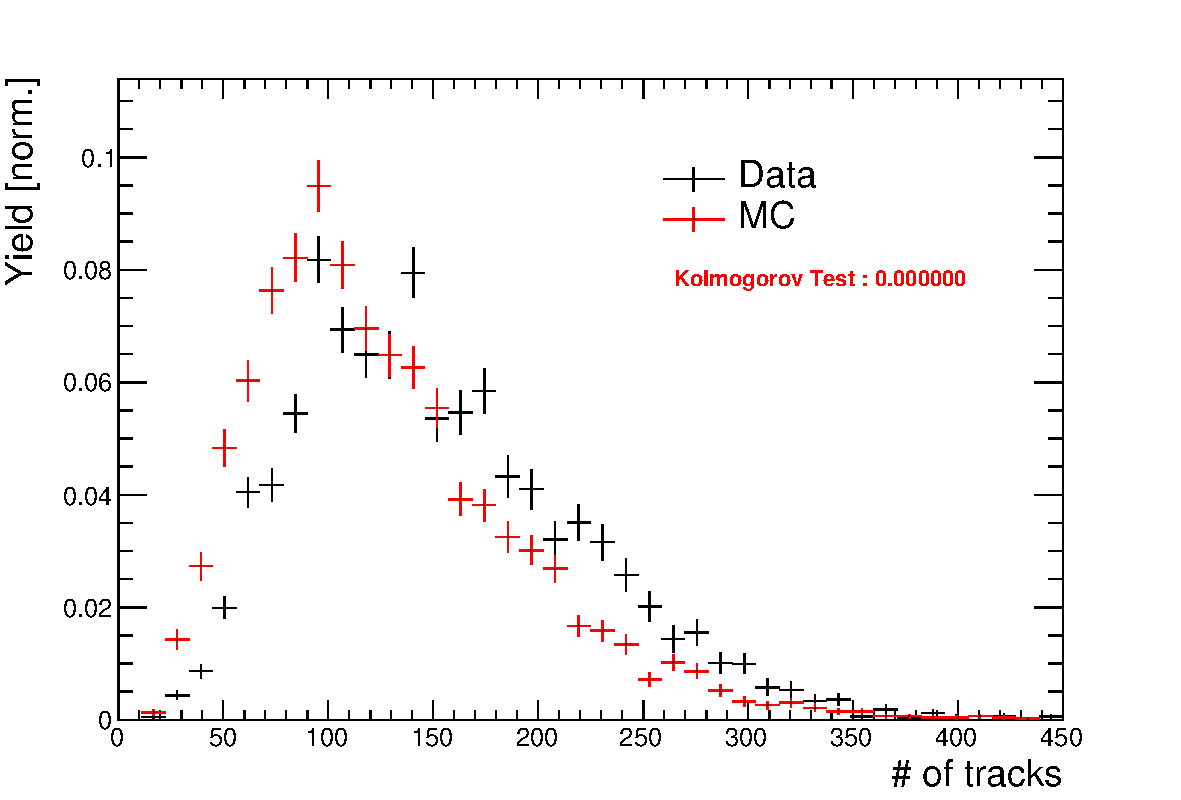
\includegraphics[height=6.cm,width=0.45\textwidth]{figs/nTracks.pdf}
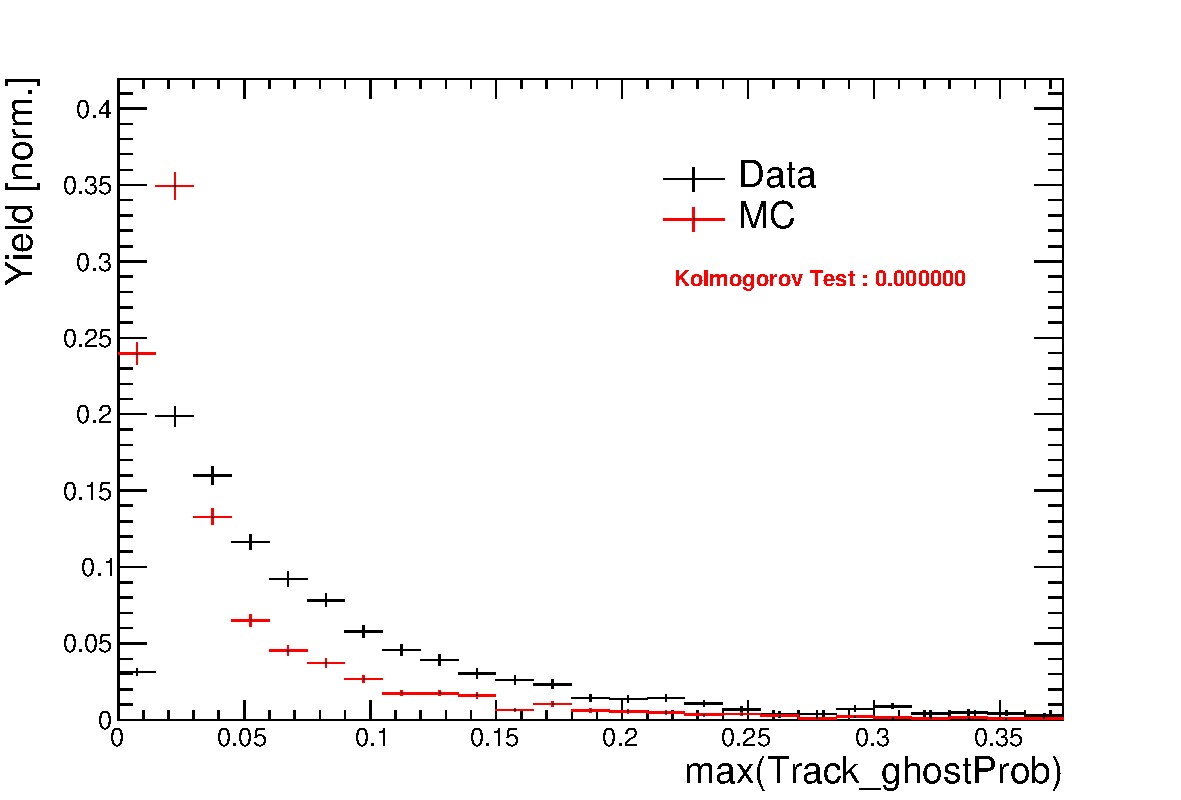
\includegraphics[height=6.cm,width=0.45\textwidth]{figs/max_ghostProb.pdf}
\caption{Comparison between the distribution of (left) the number of tracks and (right) the maximum ghost probability over all tracks in (black) data and (red) simulation.}
\label{fig: MCbeforeWeighting}
\end{figure}


In both cases, the distributions differ significantly. Therefore, we reweight the MC samples using those two variables. 
The reweighting is done successively, e.g. we perform two 1D weighting processes, where we equalize the respective MC distribution to the observed distribution in data.  
All distributions of observables used in the BDT training, before and after the reweighting procedure, are shown in the Appendix \ref{sec: mcvdata}.                 
